\subsection{2024/3/4 问题}
refine流程
\begin{itemize}
	\item 先将三角面保存投影到相机的归一化平面中,并且开启深度检测,将深度缓存提取出来获取三角面的深度图
	\item 在创建一张faceinfo的面信息图,面信息包括图元id、c值是$(1,0,0)、(0,1,0)、(0,0,1)$
	\item 在第二张图片中,重投影深度较小的像素值会写入到重投影图中。
	\item 基于重投影中,重投影深度比较小的点,计算一张深度梯度图
	\item 在两张途中ncc值较小的两个像素输出一个相关性(correlation)梯度值
	\item 顶点位置-(顶点三角面法向*梯度值)
\end{itemize}

\begin{figure}[h]
    \centering
    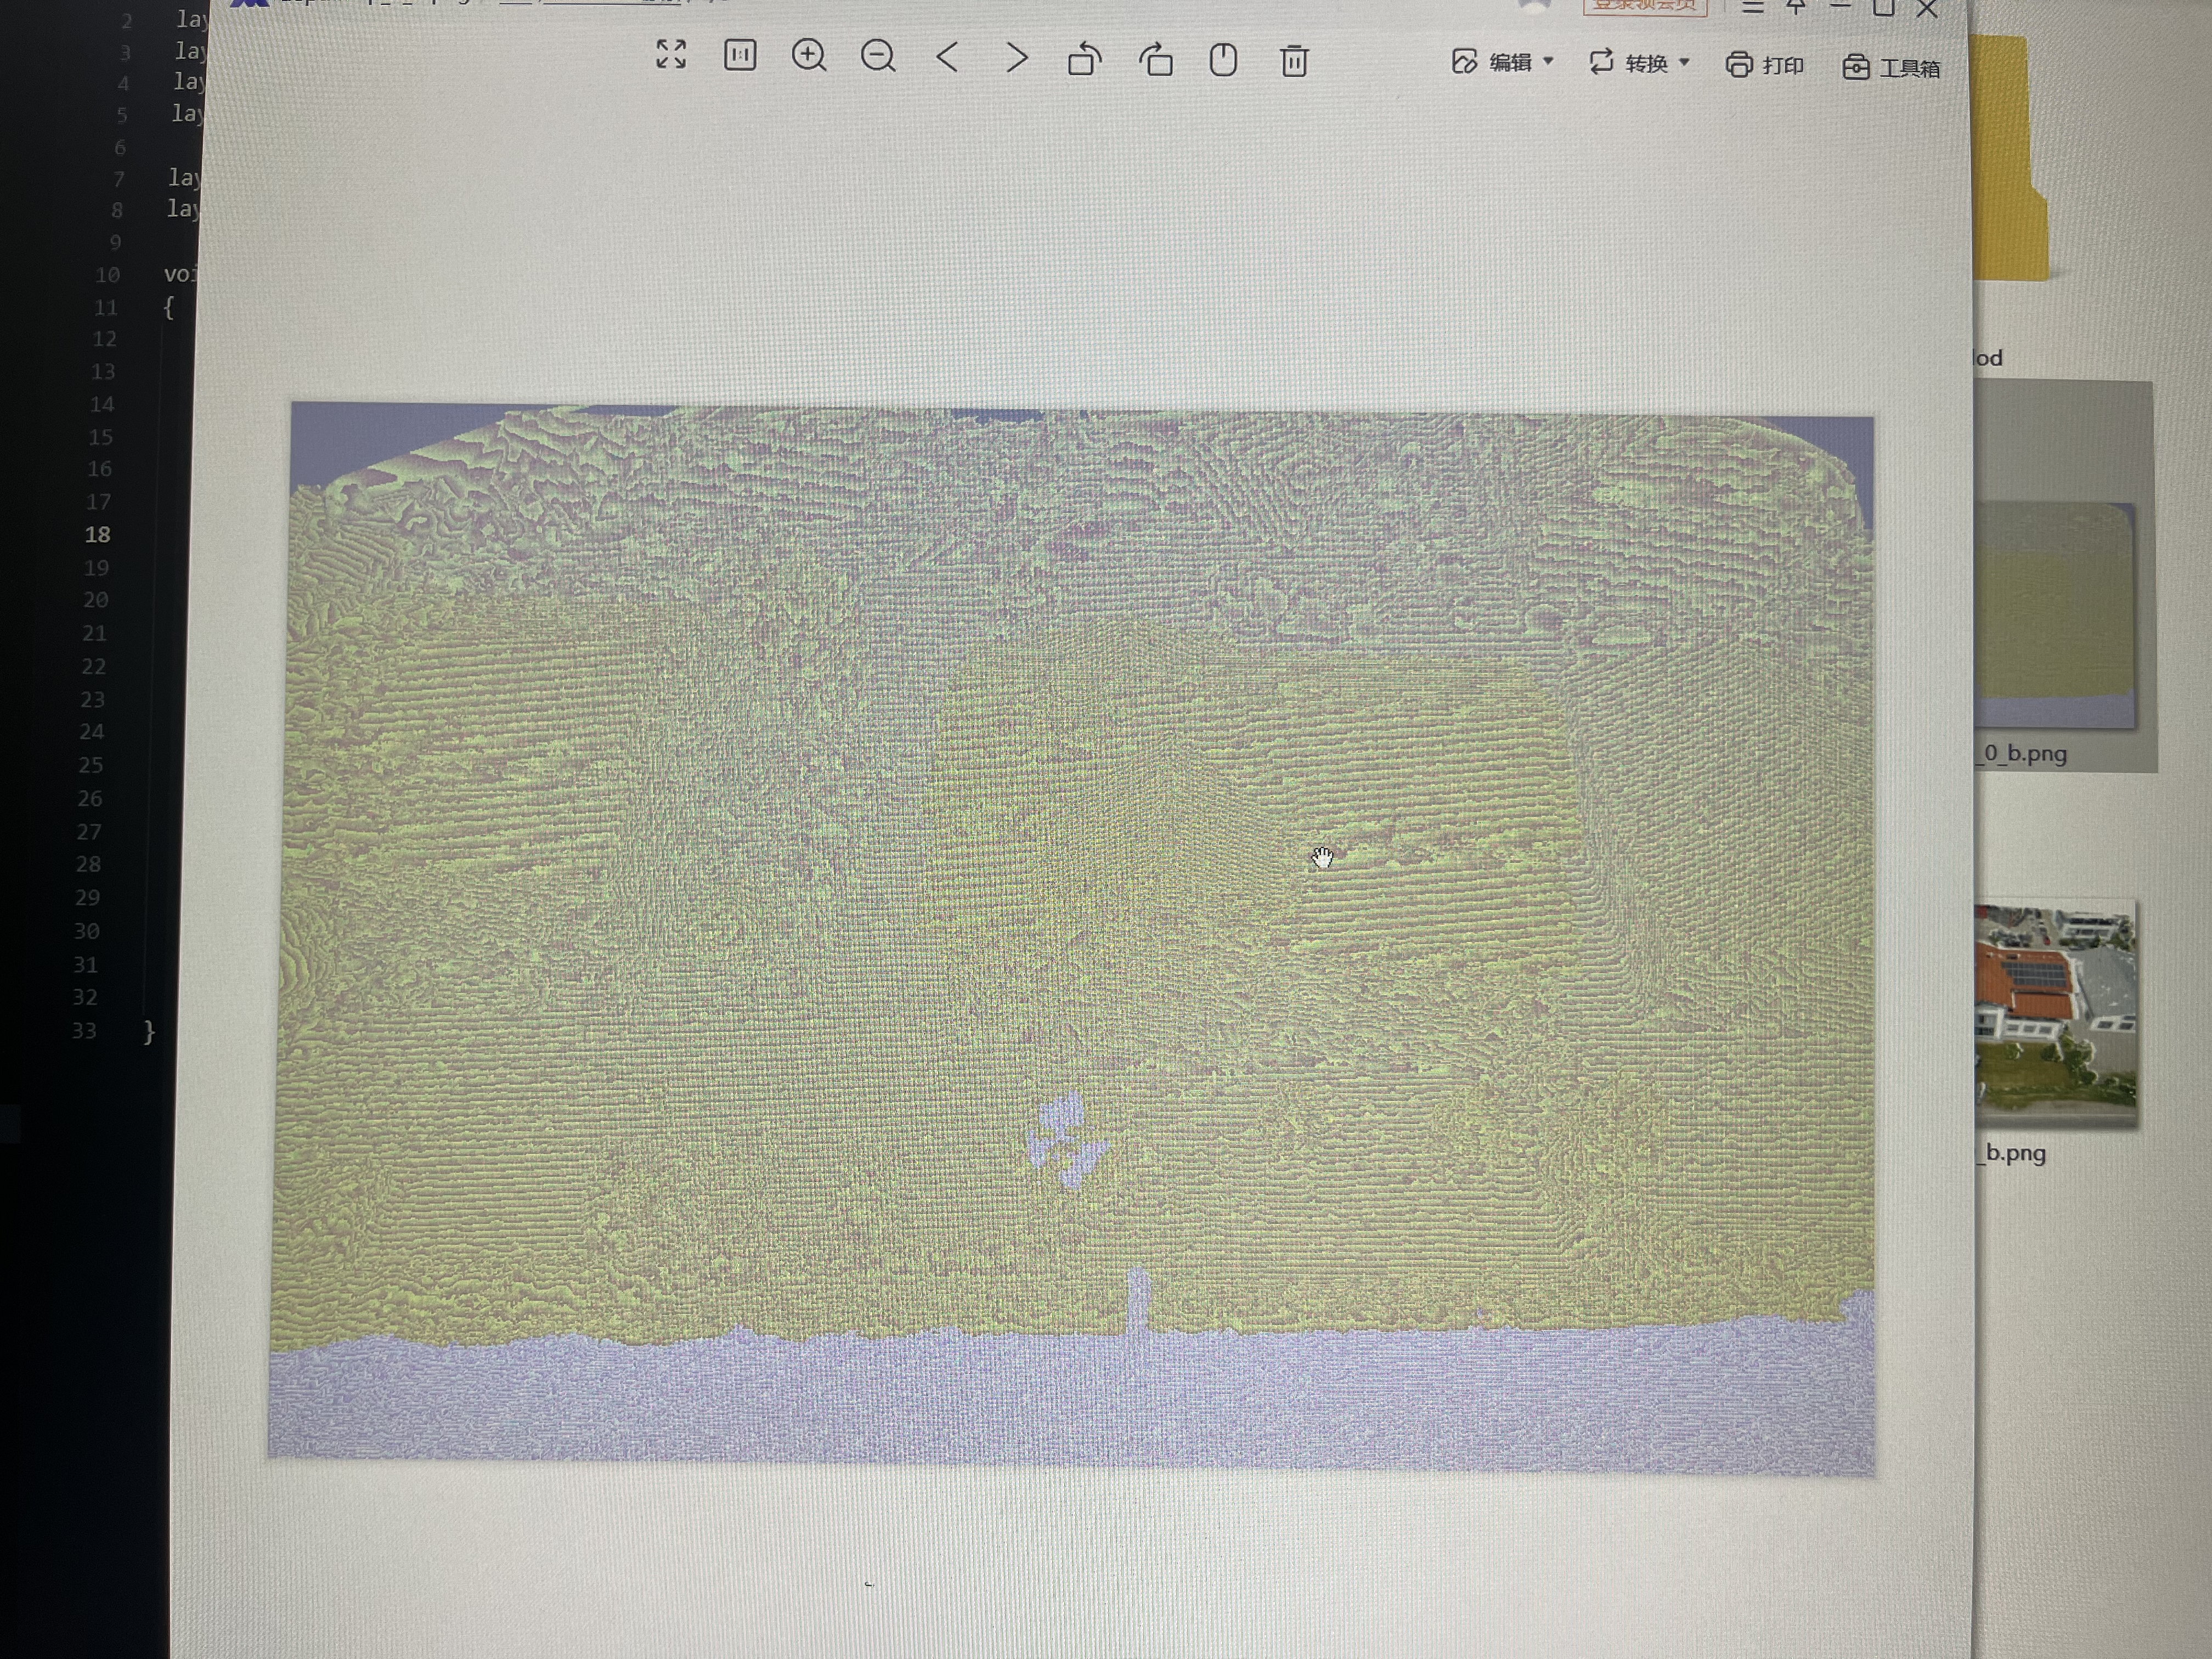
\includegraphics[height=5in]{depthmap.jpg}
    \caption{深度图}
\end{figure}

\begin{figure}[h]
    \centering
    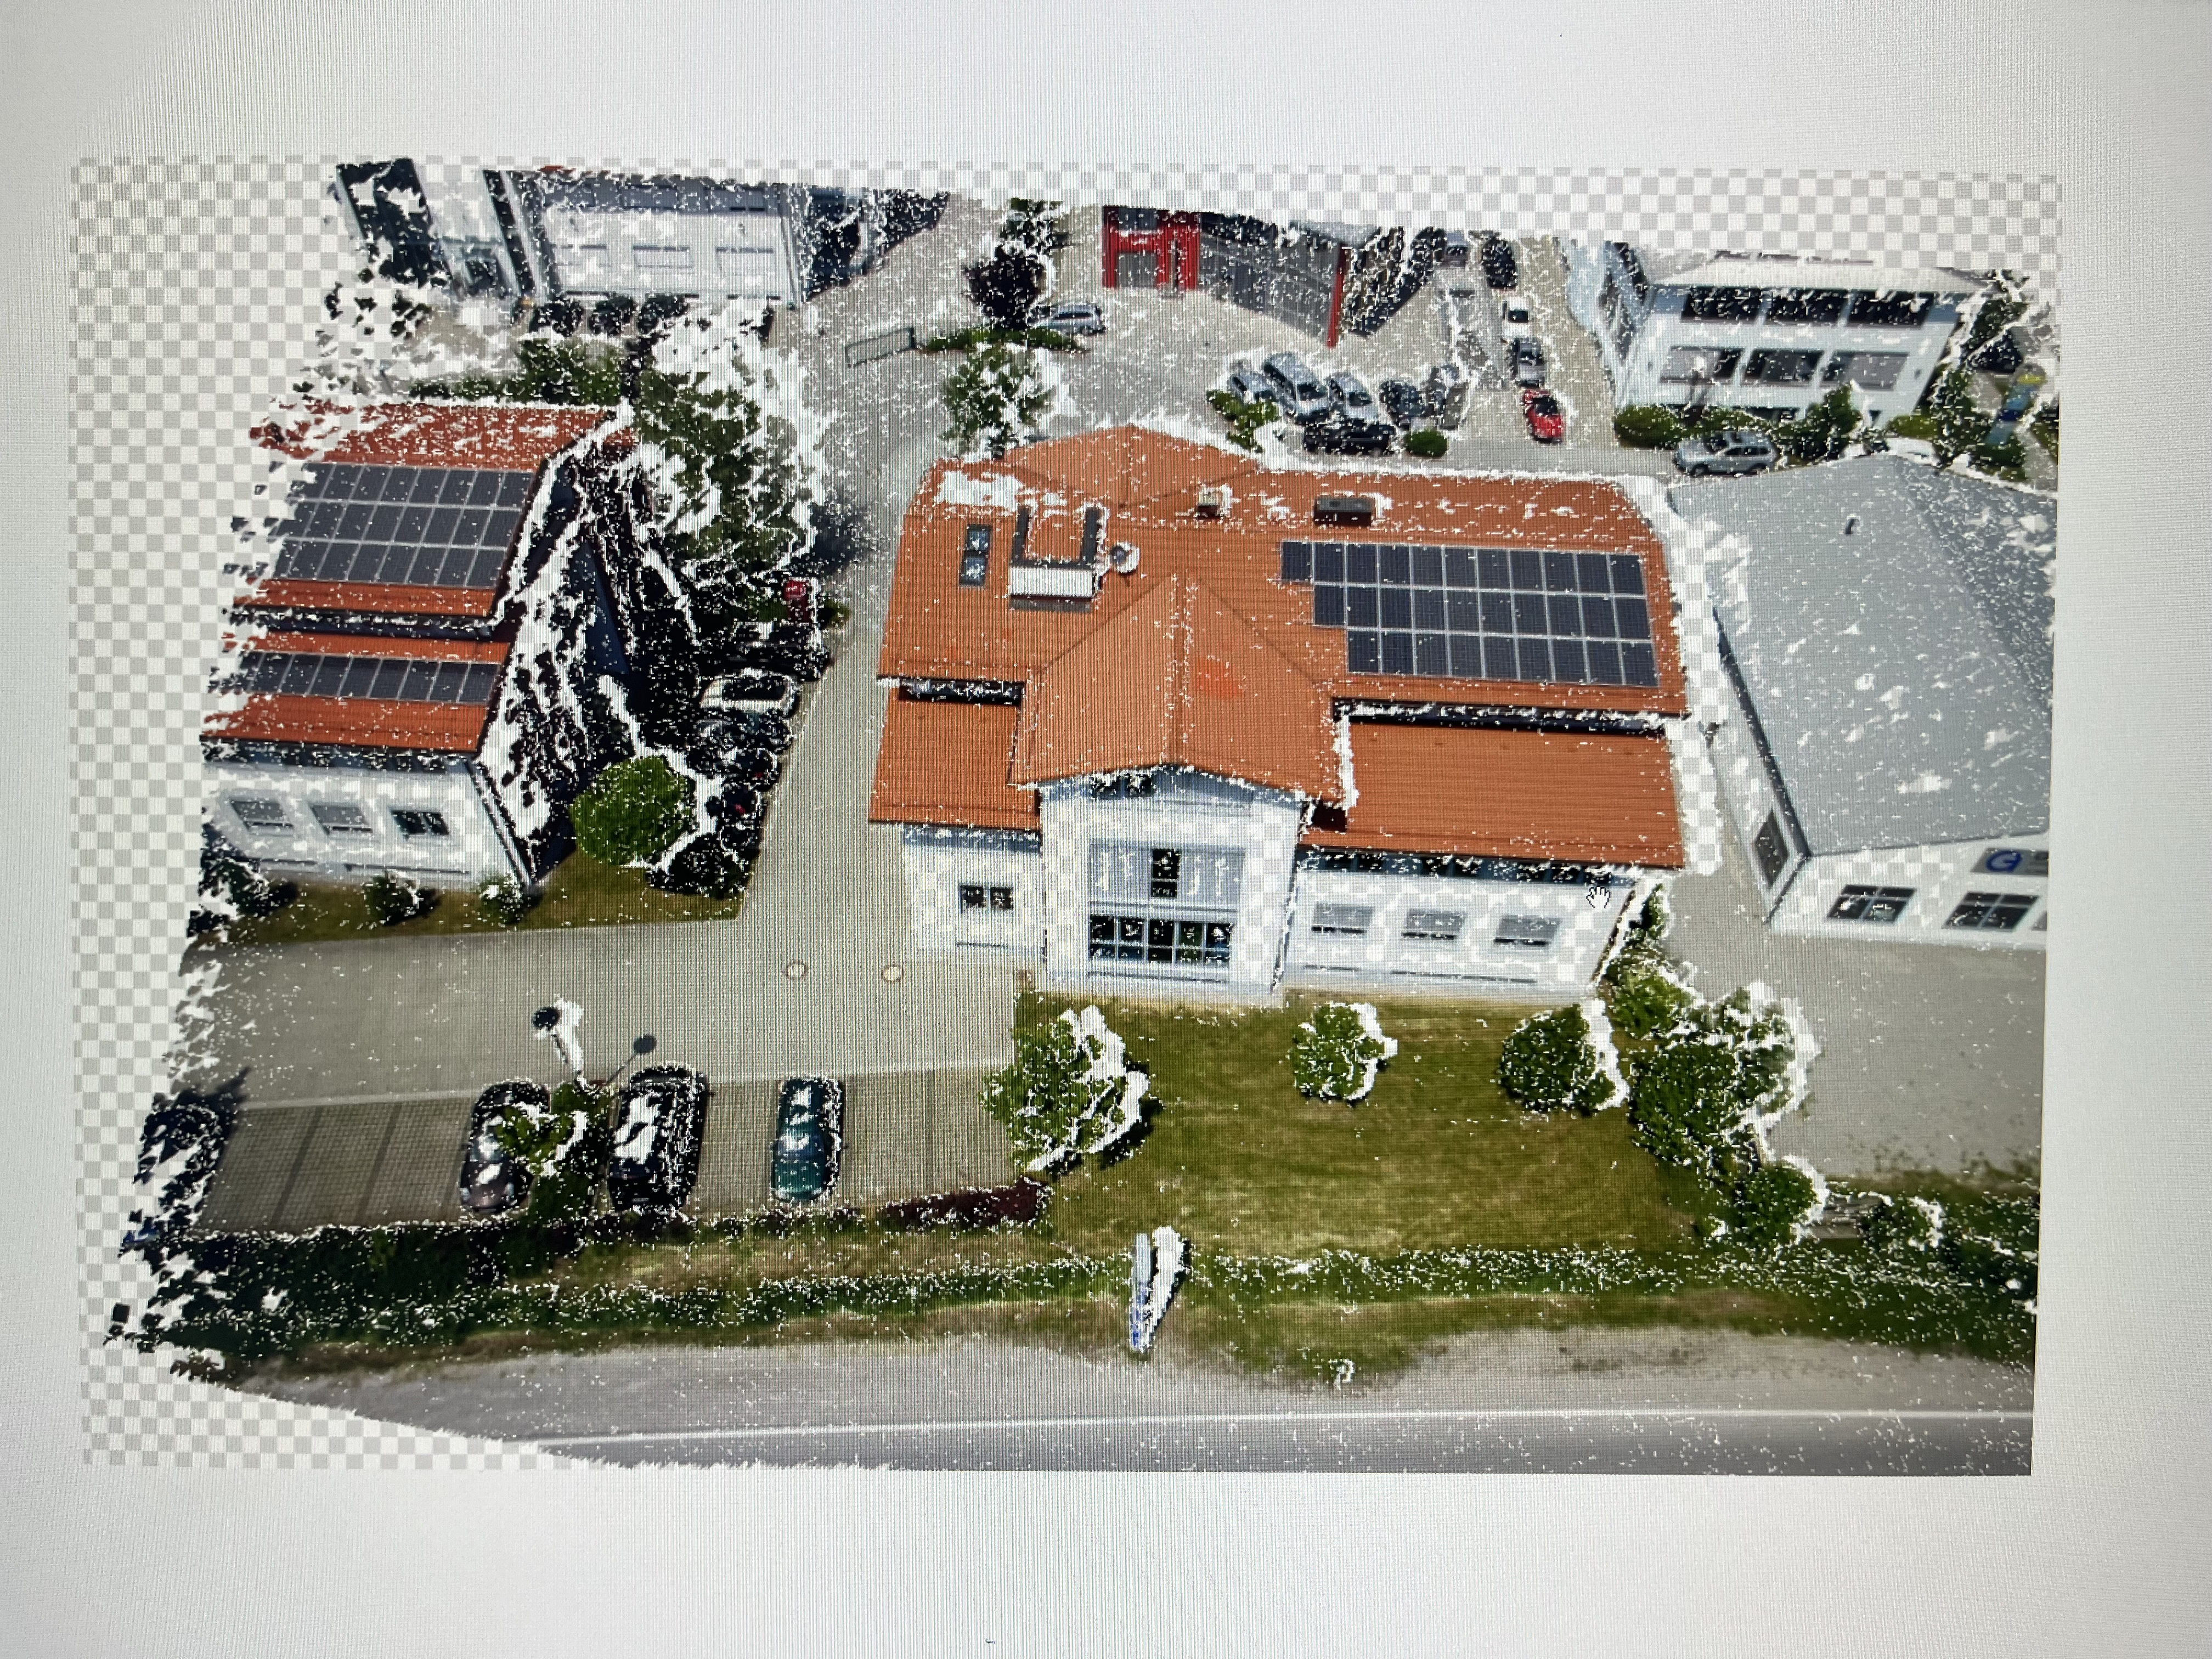
\includegraphics[height=5in]{reprojection.jpg}
    \caption{重投影}
\end{figure}

\begin{figure}[h]
    \centering
    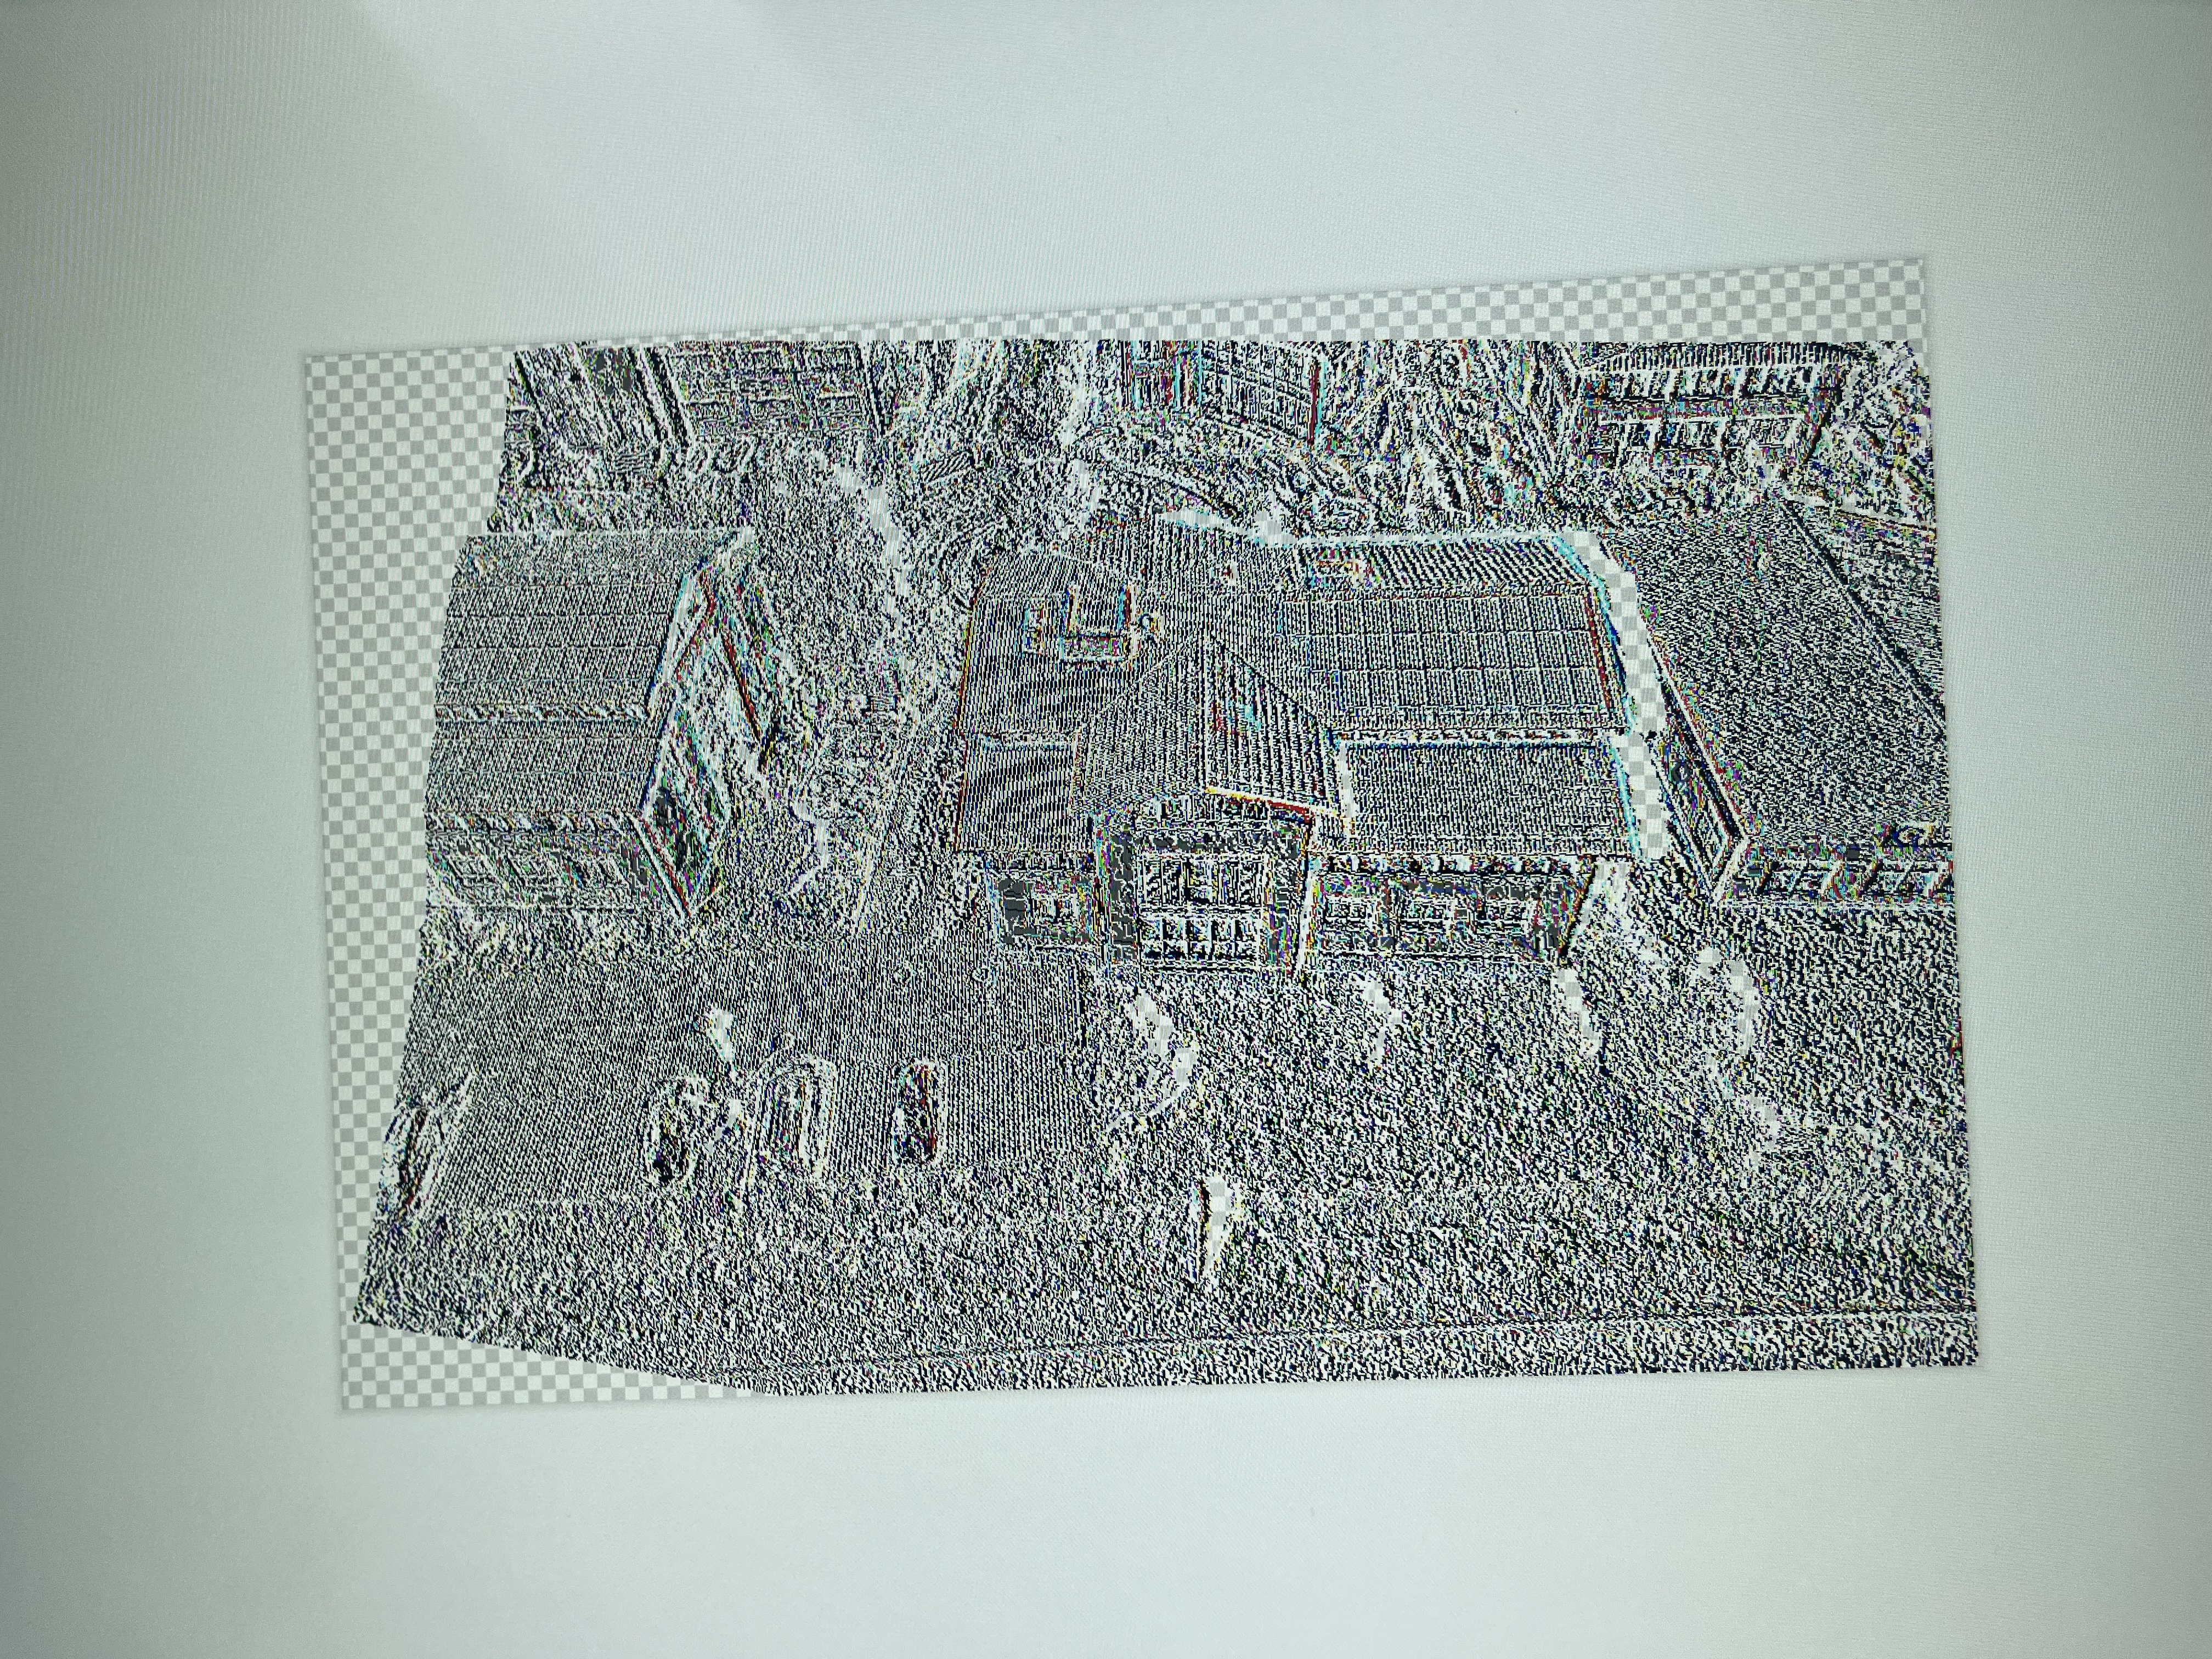
\includegraphics[height=5in]{variation.jpg}
    \caption{深度梯度}
\end{figure}

\begin{itemize}
	\item 什么是ProjectionVulkanMatrix矩阵,看起来好像是投影到相机归一化平面的矩阵
	\item 什么是TextureMatrix矩阵?
\end{itemize}

会议记要

密集匹配:平面扫掠+acmm

三个线程:

\begin{itemize}
	\item 图像校正+图像金字塔创建
	\item gpu平面扫掠密集匹配
	\item 保存密集点云
\end{itemize}


构网

纯CPU

refine

GPU加速

\begin{itemize}
	\item 快速:两个分辨率(1/4和1/2)
	\item 普通和精细:三个分辨率
\end{itemize}

网格简化

塌边简化算法,平面简化限制,可做到保留细节,对平面简化尽量用大的三角面


纹理贴图:
两个代码:
mvs原始代码,打分计算利用densecloud的相对。通过ncc相对最大的相对保留,遮挡+分辨率+模糊进行打分,打分机制

一个模型多贴图,大部分一个贴图一个模型。

lodmesh:


2.5维的dom或者dsm


像素记录那个位置的高程图。